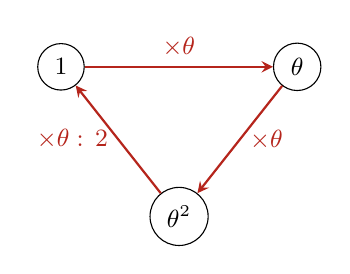
\begin{tikzpicture}[>=stealth,font=\small]
\node[draw,circle] (a) at (0,0) {$1$};
\node[draw,circle] (b) at (3,0) {$\theta$};
\node[draw,circle] (c) at (1.5,-1.9) {$\theta^2$};
\draw[->,BrickRed,thick] (a)--node[above] {$\times\theta$}(b);
\draw[->,BrickRed,thick] (b)--node[right] {$\times\theta$}(c);
\draw[->,BrickRed,thick] (c)--node[left] {$\times\theta:\,2$}(a);
\end{tikzpicture}
